\documentclass{standalone}
% fonts
\usepackage{mathpazo} % math & rm
\linespread{1.05} % Palatino needs more leading (space between lines)
% tikz
\usepackage{tikz}
%\usetikzlibrary{positioning,shapes}
\usepackage{pgfplots}

% this data is from the out.txt file in the maze stuff

\begin{document}
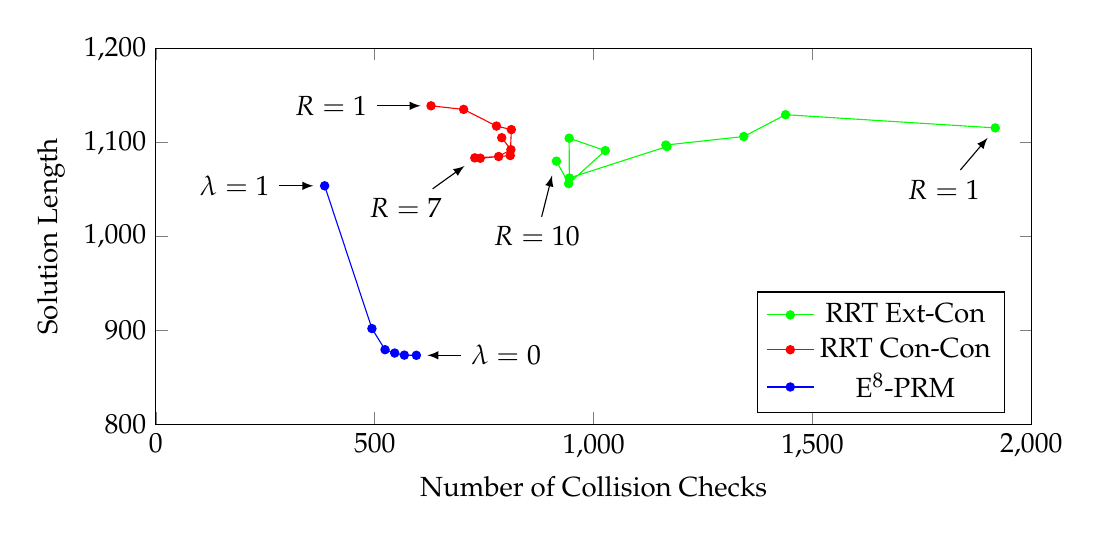
\begin{tikzpicture}
\tikzset{>=latex} % arrow heads

\begin{axis}[
   xlabel=Number of Collision Checks,
   ylabel=Solution Length,
   ylabel near ticks,
   xlabel near ticks,
   xmin=0,xmax=2000,
   xtick={0, 500, 1000, 1500, 2000},
   ymin=800,ymax=1200,
   width=5in,height=2.5in,
   legend pos=south east]

   \addplot[mark=*,green,mark size=1.5] plot coordinates {
      (1917.5,1115.59610746)
      (1438.5,1129.66416654)
      (1343.0,1106.43355199)
      (1165.0,1097.36500054)
      (1167.5,1095.73819015)
      (944.5,1062.24829858)
      (944.0,1104.68120359)
      (1026.5,1091.40824884)
      (943.0,1056.31474215)
      (915.0,1080.20385347)
   };
   \addlegendentry{RRT Ext-Con}
   
   \addplot[mark=*,red,mark size=1.5] plot coordinates {
      (628.5,1139.1373789)
      (703.0,1135.31791638)
      (778.0,1117.56601508)
      (812.0,1113.80283371)
      (809.5,1086.1570696)
      (741.0,1083.29576935)
      (728.5,1083.67831841)
      (783.0,1085.10024026)
      (811.0,1092.4306706)
      (790.0,1105.16362669)
   };
   \addlegendentry{RRT Con-Con}

   \addplot[mark=*,blue,mark size=1.5] plot coordinates {
      (595.0,873.34651418)
      (567.5,873.536357673)
      (545.5,875.763893691)
      (523.5,879.312768943)
      (493.5,901.843256314)
      (385.5,1053.91187555)
   };
   \addlegendentry{E$^8$-PRM}
   
   \node (labl0) at (axis cs:800,873.34651418) {$\lambda=0$};
   \draw[->] (labl0) -- (axis cs:620,873.34651418);
   
   \node (labl1) at (axis cs:180,1053.91187555) {$\lambda=1$};
   \draw[->] (labl1) -- (axis cs:360,1053.91187555);
   
   \node (labccr1) at (axis cs:400,1139.1373789) {$R=1$};
   \draw[->] (labccr1) -- (axis cs:605,1139.1373789);
   
   \node (labccr7) at (axis cs:570,1030) {$R=7$};
   \draw[->] (labccr7) -- (axis cs:705,1075);
   
   \node (labecr1) at (axis cs:1800,1050) {$R=1$};
   \draw[->] (labecr1) -- (axis cs:1900,1105);
   
   \node (labecr10) at (axis cs:870.0,1000) {$R=10$};
   \draw[->] (labecr10) -- (axis cs:905.0,1065);
   
\end{axis}

\end{tikzpicture}
\end{document}
